\chapter{Membangun Model Prediksi}

\section{Teori}
	\subsection{Binary Classification}
	Binary Classification merupakan klasifikasi yang memiliki 2 label kelas. Biasanya melibatkan satu kelas yang merupakan keadaan normal dan kelas lainnya yang merupakan keadaan abnormal atau dapat berarti binary classification berupa kelas positif dan kelas negatif. Contohnya, pada email terdeteksi spam email, ada keadaan dimana email tersebut dapat berupa spam atau bukan.  Misalnya bukan spam berarti keadaan normal dan spam berarti keadaan abnormal. Kelas dengan keadaan normal atau positif diberi label kelas 0 dan kelas dengan keadaan abnormal atau negatif diberi label kelas 1. 
	\newline Algoritma yang digunakan untuk binary classification yaitu :
	\begin{enumerate}
		\item Logistic Regression
		\item K-Nearest Neighbors
		\item Decision Trees
		\item Support Vector Machine
		\item Naive Bayes
	\end{enumerate}

	\begin{figure}[!htbp]
		\centering
		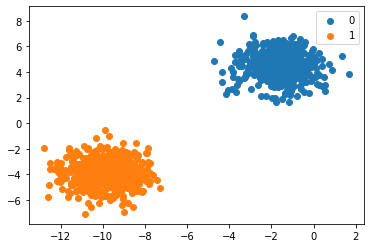
\includegraphics[width=9cm,height=7cm]{figures/Binary_Classification.png}
		\caption{Binary Classification}
		\label{penanda}
	\end{figure}

	\subsection{Supervised Learning, Unsupervised Learning dan Clustering }
	\begin{enumerate}
        \item Supervised Learning
        \newline Supervised Learning merupakan teknik belajar model dimana sebuah model akan diberi data dan setiap data tersebut akan diberi label. Dalam supervised learning terdapat data training yang menjadi tempat semua data dimana data training berupa input data atau target data yang diinginkan kemudian dilatih untuk dapat melakukan prediksi  dalam menjawab target data. Data tersebut akan diuji dan dibandingkan dengan prediksi pada data test. Supervised learning juga dapat didefinisikan sebagai operasi machine learning yang digunakan untuk data dimana ada pemetaan yang tepat antara data input dan output. Kumpulan data akan diberi label yang berarti algoritma akan mengidentifikasi secara eksplisit dan akan melakukan prediksi atau klasifikasi yang sesuai. 

		\begin{figure}[!htbp]
			\centering
			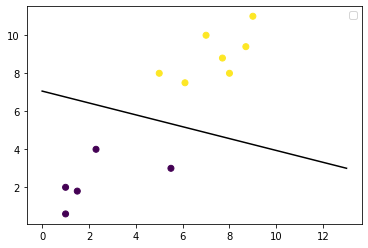
\includegraphics[width=9cm,height=7cm]{figures/SVM_LinearKernel.png}
			\caption{Supervised Learning : SVM Model Using Linear Kernel}
			\label{penanda}
		\end{figure}

        \item Unsupervised Learning
        \newline Unsupervised Learning merupakan operasi machine learning yang mempelajari sebuah pola data tanpa memerlukan target data. Unsupervised Learning hanya memerlukan data input dan menemukan pola serta insight penting dari data. Proses ini biasa disebut dengan data mining. Pada Unsupervised Learning data tidak memiliki label secara eksplisit dan mampu belajar dari data dengan menemukan pola implisit. Unsupervised Learning tidak menggunakan data training dan hanya bergantung pada data test sehingga tidak dapat dilakukan evaluasi pada model. Unsupervised Learning dievaluasi secara subjektif untuk dapat mengetahui bahwa prediksi yang dilakukan sudah sesuai. 

		\begin{figure}[!htbp]
			\centering
			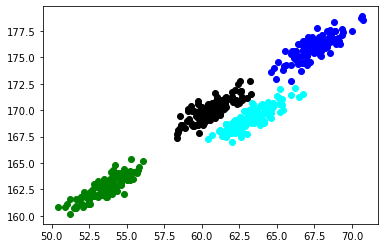
\includegraphics[width=9cm,height=7cm]{figures/Gaussian_Mixture.png}
			\caption{Unsupervised Learning : Gaussian Mixture Model}
			\label{penanda}
		\end{figure}


        \item Clustering
        \newline Clustering merupakan sebuah teknik machine learning yang digunakan untuk mengelompokkan data tidak berlabel atau merupakan sebuah metode yang digunakan untuk pengelompokkan data secara otomatis dengan membagi kumpulan data menjadi beberapa kelompok sesuai kesamaannya. Algoritma pengelompokkan digunakan untuk memproses objek data yang tidak di klasifikasi ke dalam kelompok yang diwakili dengan struktur atau sebuah pola dalam informasi 
        \end{enumerate}

	\subsection{Evaluasi dan Akurasi}
	Evaluasi merupakan kegiatan yang dilakukan untuk mengukur seberapa baik sebuah model dapat bekerja dengan menghitung akurasinya. Akurasi merupakan ukuran atau persentase data yang diklasifikasikan dengan benar. Akurasi klasifikasi juga dapat berarti membagi jumlah prediksi benar terhadap total prediksi. Dalam model klasifikasi, dapat diprediksi nilai terbesar dan memberikan akurasi yang tinggi serta model yang dihasilkan dapat memprediksi nilai yang salah. Sehingga dalam hal ini dibutuhkan adanya metrik evaluasi yang dapat mengukur peforma dari model klasifikasi yang sudah dibuat. Metrik yang digunakan adalah Precision, Recall dan Confusion Matrix.

	\subsection{Confusion Matrix}
	Confusion Matrix atau disebut juga dengan Error Matrix pada dasarnya akan memberikan informasi mengenai perbandingan hasil dari klasifikasi yang dilakukan oleh model atau sistem dengan hasil sebenarnya. Confusion Matrix berbentuk tabel matrix yang akan menggambarkan kinerja dari model klasifikasi pada data uji yang nilai sebenarnya diketahui.
	\newline 
	\textbf {Berikut adalah contoh dari confusion matrix :}
	\begin{enumerate}
		\item Accuracy
		\item Precision (Positive Predictive Value)
		\item Recall atau Sensitivity (True Positive Rate)
	\end{enumerate}
	\textbf {Cara membuat dan membaca confusion matrix}
	\begin{enumerate}
		\item Tentukan pokok permasalahan atau menggunakan dataset, misalnya data pasien covid
		\item Membagi dataset serta membuat model prediksi menggunakan Decision Tree. Dataset dibagi menjadi dua yaitu data latiih dan data uji. Data latih digunakan untuk melatih model yang dibuat dan evaluasi akan dilakukan pada data uji. 
		\item Evaluasi model menggunakan confusion matrix yaitu untuk mengetahui keakuratan model yang sudah dibuat menggunakan performance metrics seperti: accuracy, recall, dan precision.
	\end{enumerate}
	\begin{figure}[!htbp]
		\centering
		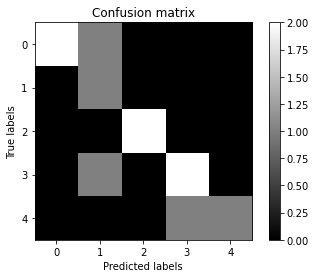
\includegraphics[width=9cm,height=7cm]{figures/confusion_matrix.png}
		\caption{Confusion Matrix}
		\label{penanda}
	\end{figure}

	\subsection{K-fold cross validation}
	K-fold cross validation merupakan model evaluasi atau prosedur yang akan memisahkan antara data training dan data testing. K-fold cross validation dapat di definisikan sebagai pengujian cross validation yang digunakan untuk menilai kinerja dari sebuah metode algoritma dengan membagi sampel data secara acak dan mengelompokkan data tersebut sebanyak nilai K k-fold.
	\begin{figure}[!htbp]
		\centering
		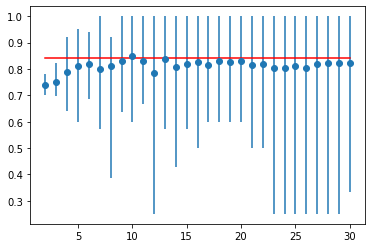
\includegraphics[width=9cm,height=7cm]{figures/kvold_validation.png}
		\caption{K-fold cross validation}
		\label{penanda}
	\end{figure}
	\newline
	\textbf {Cara kerja K-fold cross validation : }
	\begin{enumerate}
		\item Tentukan instance, dibagi menjadi N bagian atau misalnya ada 10 data dan akan dilakukan K-fold cross validation pada data tersebut.
		\item Data dibagi menjadi data testing untuk pengujian pada model dan data training untuk melatih model. 
		\item Menentukan nilai K, misalnya dalam hal ini ditentukan nilai K = 10 dimana data tersebut nantinya akan ada 10 lipatan atau disebut dengan fold
	\end{enumerate}

	\subsection{Decision Tree}
	Decision Tree merupakan metode penbelajaran non parametrik yang digunakan untuk klasifikasi dan regresi. Tujuan dari decision tree adalah membuat model yang akan memprediksi nilai variable dengan mempelajari aturan keputusan sederhana yang disimpulkan dari sebuah fitur data. Decision tree merupakan struktur yang sama seperti diagram alur dimana simpul internal sebagai fitur atau atribut, cabang sebagai aturan dan keputusan, serta setiap simpul daun akan mewakili hasilnya.
	\begin{figure}[!htbp]
		\centering
		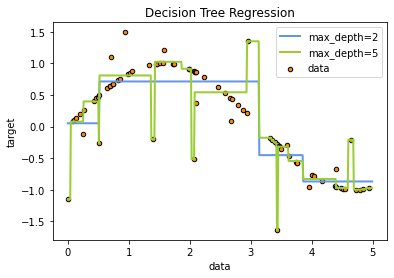
\includegraphics[width=9cm,height=7cm]{figures/decision_tree_regresi.png}
		\caption{Decision Tree}
		\label{penanda}
	\end{figure}

	\subsection{Information Gain dan Entropi}
	\begin{enumerate}
	\item Entropi
	\newline Sebuah objek yang di akan di klasifikasikan ke dalam decision tree harus di uji nilai entropinya. Entropi merupakan ukuran dari informasi yang dapat mengetahui karakteristik  dari dari impuryt ,dan homogenity dari sekumpulan data. Entropi juga merupakan jumlah bit yang diperkirakan akan dibutuhkan untuk mengekstrak suatu kelas dari data acak pada suatu ruang sampel. Dari nilai entropi tersebut kemudian akan dihitung information gain masing-masing atribut. 

	\item Information Gain
	\newline Kemudian setelah mendapatkan nilai entropi untuk suatu kumpulan data, maka akan diukur efektivitas nya atau disebut dengan information gain. Information gain digunakan untuk mengukur seberapa besar relevan atau pengaruh sebuat feature terhadap hasil pengukuran. Information Gain dikenal juga dengan sebutan Mutual Information dalam kasus untuk mengetahui dependency antara dua variable (x,y).
	\end{enumerate}


\section{Praktikum}
	\subsection{Scikit-Learn}
\begin{enumerate}

\item Load Dataset student-mat.csv
\newline Digunakan untuk import module pandas dan mendefinisikan variable "bandung" yang akan memanggil dataset yang diambil dari student-mat.csv.
\begin{figure}[!htbp]
	\centering
	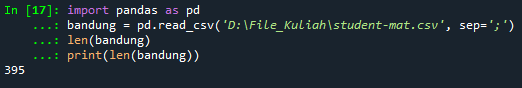
\includegraphics[width=11cm,height=2cm]{figures/load_dataset.png}
	\caption{Load Dataset}
	\label{penanda}
\end{figure}

\item Generate Binary Label
\newline Bagian ini akan mendeklarasikan pass/fail data berdasarkan G1+G2+G3 dengan ketentuan nilai pass = 30 dan pada variable bandung dideklarasikan jika baris dengan G1+G2+G3 ditambahkan, dan hasilnya sama dengan 35 maka axis nya 1.
\begin{figure}[!htbp]
	\centering
	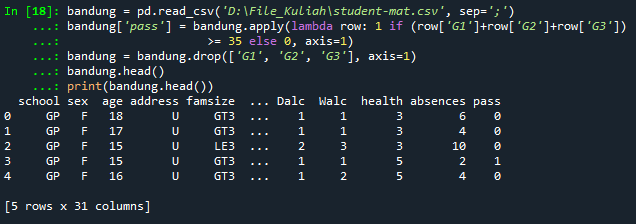
\includegraphics[width=13cm,height=5cm]{figures/binary_label.png}
	\caption{Generate Binary Label}
	\label{penanda}
\end{figure}

\item Use one-hot encoding on categorical columns 
\newline One-hot encoding merupakan proses dimana sebuah variable kategorikal dikonversikan menjadi bentuk yang dapat disediakan oleh algoritma Machine Learning untuk dapat melakukan pekerjaan yang lebih baik dalam memprediksi. Disini menggunakan fungsi panda pdgetdummies untuk jenis kelamin, sekolah, alamat dan lainnya. Metode head ini digunakan untuk mengembalikan baris n atas 5 secara default dari frame atau seri datanya.
\begin{figure}[!htbp]
	\centering
	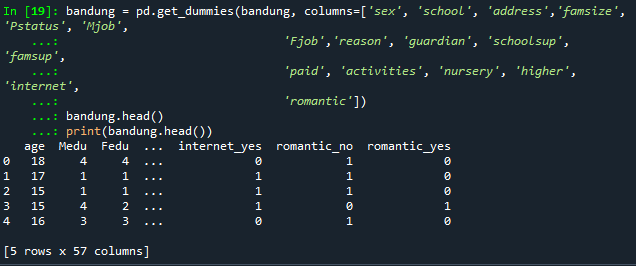
\includegraphics[width=12cm,height=4cm]{figures/one_hot.png}
	\caption{Use one-hot encoding on categorical columns}
	\label{penanda}
\end{figure}

\item Shuffle Rows
\newline Digunakan untuk mengembalikkan sample secara acak item dari objek. Terdapat train dan test yang digunakan untuk membagi train, test dan kemudian dibagi lagi train ke validasi dan test. kemudian di import sebuah modul numpy sebagai np yang digunakan untuk mengembalikan nilai passing dari pelajar dan dari keseluruhan dataset dengan menggunakan print.
\begin{figure}[!htbp]
	\centering
	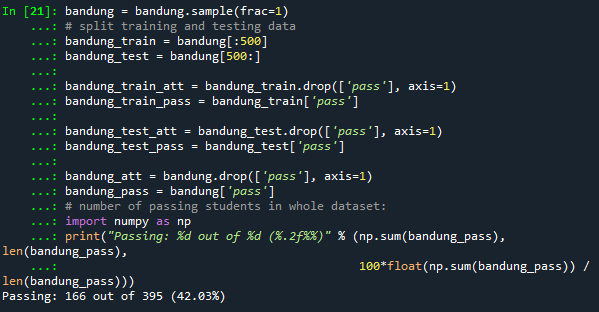
\includegraphics[width=12cm,height=6cm]{figures/shuffle_rows.png}
	\caption{Shuffle Rows}
	\label{penanda}
\end{figure}

\item Fit a decision tree
\newline Import modul tree dari library scikit-learn. Kemudian definisikan variable bandung menggunakan decision classifier. Di dalam variable bandung terdapat criterion yang merupakan suatu fungsi untuk mengukur kualitas split. Agar decision tree classifier dapat di jalankan maka gunakan perintah fit
\begin{figure}[!htbp]
	\centering
	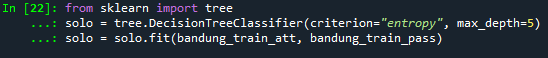
\includegraphics[width=12cm,height=1cm]{figures/decision_tree.png}
	\caption{Fit a decision tree}
	\label{penanda}
\end{figure}

\item Visualize tree
\newline Graphviz merupakan perangkat lunak visualisasi grafik objek open source. Visualisasi grafik merupakan cara untuk mewakili informasi struktural sebagai diagram grafik dan jaringan abstrak. treeexportgraphviz merupakan sebuah fungsi yang akan menghasilkan representasi Graphviz dari decision tree,kemudian ditulis kedalam out file, sehingga akan ditampilkan sebuah diagram grafik bercabang.
\begin{figure}[!htbp]
	\centering
	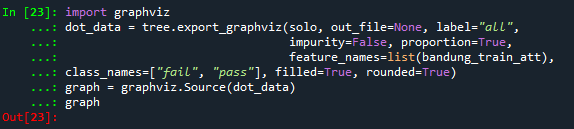
\includegraphics[width=11cm,height=3cm]{figures/graphviz.png}
	\caption{Visualize tree}
	\label{penanda}
\end{figure}
\begin{figure}[!htbp]
	\centering
	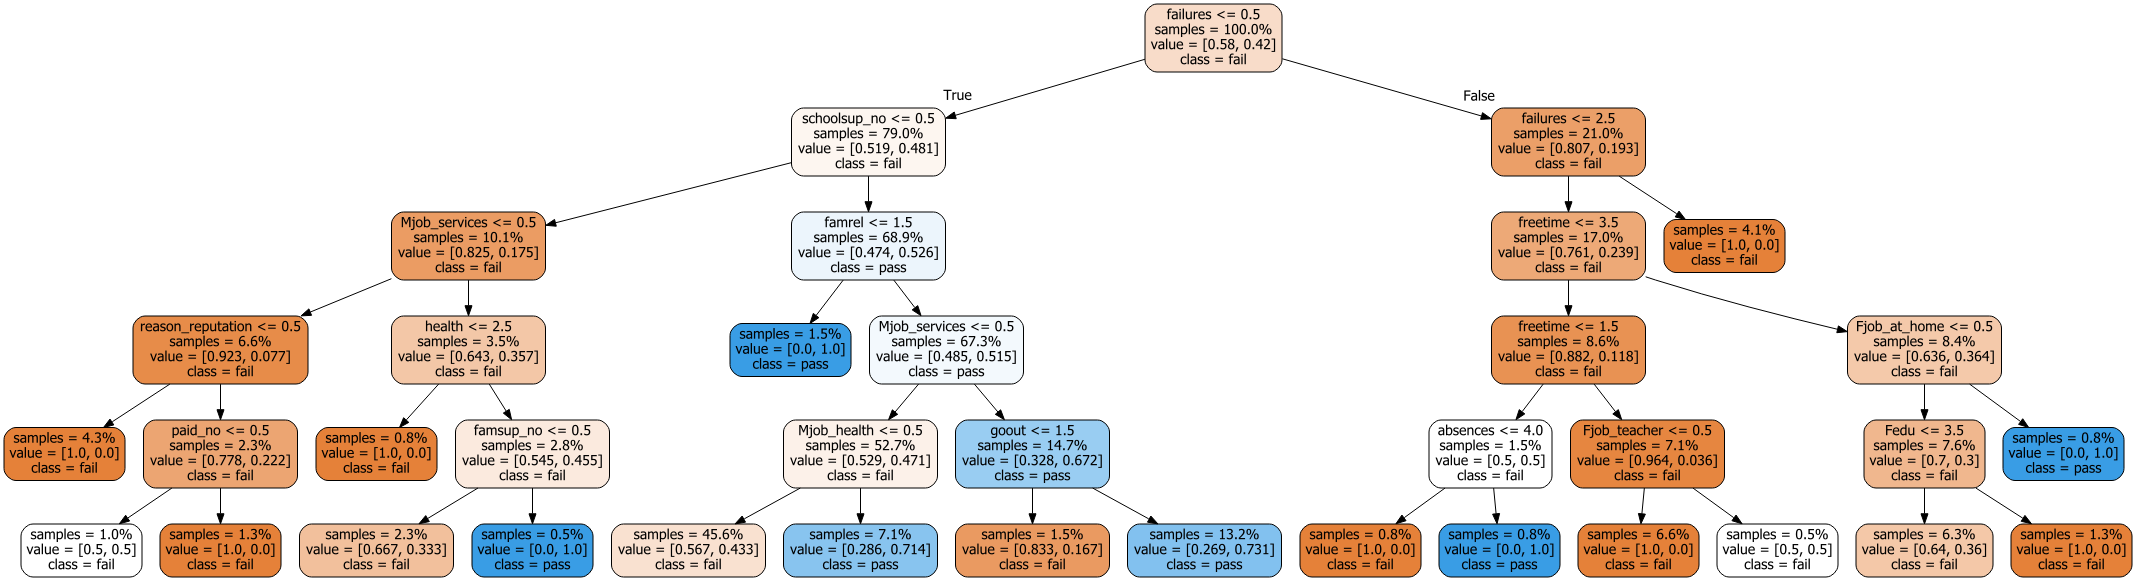
\includegraphics[width=17cm,height=5cm]{figures/visualize_tree.png}
	\caption{Visualize tree - graph}
	\label{penanda}
\end{figure}

\item Save Tree
\newline TREEEXPORTGRAPHVIZ merupakan sebuah fungsi yang akan menghasilkan representasi graphviz dari decision tree yang kemudian akan di tulis ke dalam sebuah outfile. Di dalam file tersebut akan disimpan classifier nya kemudian mengekspor file tersebut dengan namastudent performance kedalam folder tujuan kemudian jika salah maka akan mengembalikan nilai fail.
\begin{figure}[!htbp]
	\centering
	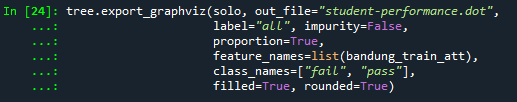
\includegraphics[width=12cm,height=2cm]{figures/save_tree.png}
	\caption{Save Tree}
	\label{penanda}
\end{figure}

\item Score
\newline Score disebut juga sebagai prediksi dan merupakan proses yang akan menghasilkan nilai berdasarkan pada model pembelajaran mesin yang terlatih dan diberi beberapa data input baru. Nilai dibuat untuk mewakili prediksi nilai di masa depan atau juga dapat mewakili kategori serta hasil yang mungkin. Dalam hal ini variable solo akan memprediksi nilai bandung test att dan test pass.

\item Evaluasi Score - Cross Val Score
\newline Pada Evaluasi Score, di script ini akan mengevaluasi score dengan menggunakan validasi silang. Dimana variable jakarta disini berisi cross val score yang merupakan fungsi pembantu pada estimator serta dataset. Kemudian akan ditampilkan score rata-rata dan kurang lebih dua standar deviasi yang mencakup 95 persen dari score.
\begin{figure}[!htbp]
	\centering
	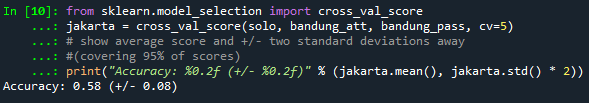
\includegraphics[width=12cm,height=2cm]{figures/cross_val_score.png}
	\caption{Evaluasi Score - Cross Val Score}
	\label{penanda}
\end{figure}

\item Max Depth
\newline Script berikut akan menunjukkan bahwa semakin banyak tree maka semakin banyak perpecahan yang dimiliki dan akan lebih banyak menangkap informasi dari data. Variable solo disini akan mendefinisikan tree kemudian variable jakarta akan mengevaluasi score nya dengan validasi silang. Kemudian akan di definisikan decision tree dengan kedalaman mulai dari 1 hingga 20 dan
merencanakan pelatihan dan menguji skor auc.
\begin{figure}[!htbp]
	\centering
	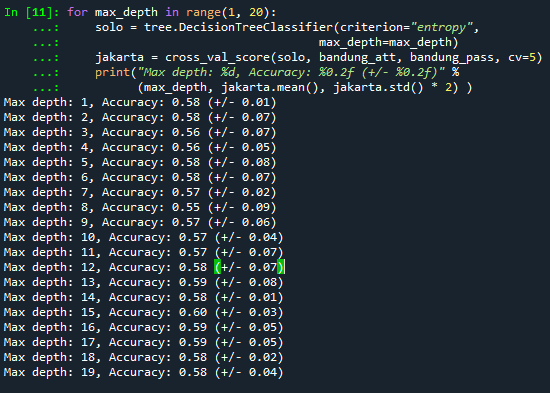
\includegraphics[width=10cm,height=7cm]{figures/max_depth.png}
	\caption{Max Depth}
	\label{penanda}
\end{figure}

\item Depth In Range
\newline Depth acc membuat array kosong dengan mengembalikan array baru menggunakan bentuk dan tipe yang diberikan, tanpa menginisialisasi entri. Dengan 19 sebagai bentuk array kosong, 3 sebagai output data-type dan float urutan kolom utama (gaya Fortran) dalam memori. Variabel solo yang akan melakukan
split score dan jakarta akan mengvalidasi score secara silang. Kemudian jakarta std yaitu menghitung standar deviasi dari data yang diberikan (elemen array) di sepanjang sumbu yang ditentukan (jika ada).
\begin{figure}[!htbp]
	\centering
	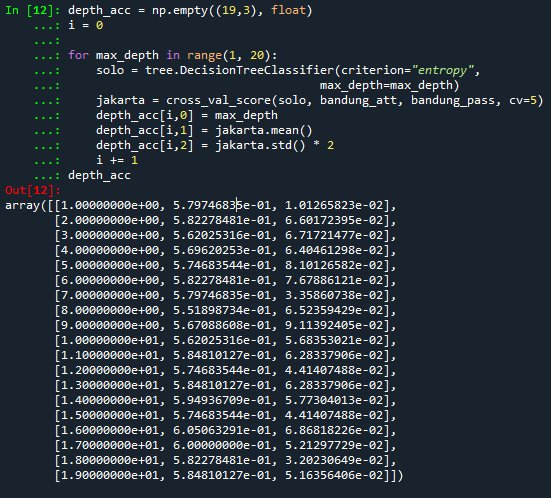
\includegraphics[width=10cm,height=8cm]{figures/depth_range.png}
	\caption{Depth In Range}
	\label{penanda}
\end{figure}

\item Matplotlib
\newline Pada Script berikut, akan di import sebuah library dari matplotlib yaitu pylot sebagai plt, fig dan ax yang menggunakan subplots untuk dapat membuat gambar serta satu set subplot. axerrorbar dalam script akan membuat error bar kemudian membuat sebuah grafik yang akan ditampilkan menggunakan perintah show.
\begin{figure}[!htbp]
	\centering
	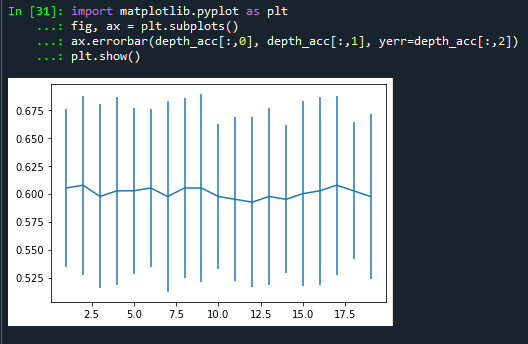
\includegraphics[width=10cm,height=6cm]{figures/matplotlib.png}
	\caption{Matplotlib}
	\label{penanda}
\end{figure}
\end{enumerate}

\section{Penanganan Error}
	\subsection{Error Graphviz}
\begin{enumerate}
	\item Berikut merupakan error yang didapat setelah menjalankan graphviz pada spyder
	\begin{figure}[!htbp]
		\centering
		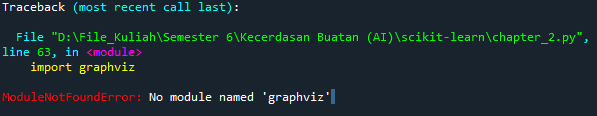
\includegraphics[width=10cm,height=2cm]{figures/error1.png}
		\caption{Error Graphviz}
		\label{penanda}
	\end{figure}
\end{enumerate}
	\textbf {Berikut merupakan Solusinya}
	\begin{enumerate}
		\item Install conda install -c anaconda pydot
		\begin{figure}[!htbp]
			\centering
			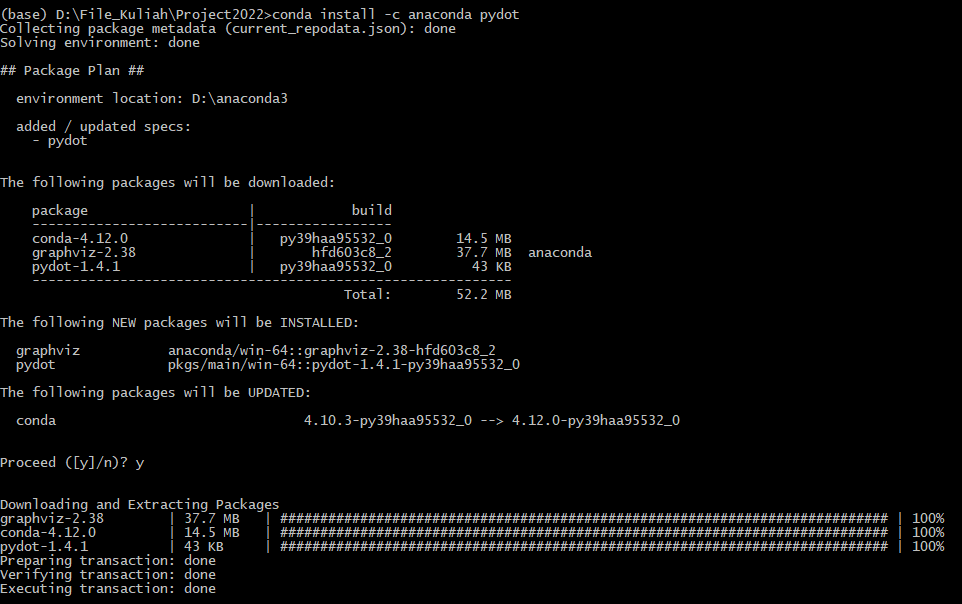
\includegraphics[width=10cm,height=6cm]{figures/solusi1_fix.png}
			\caption{Solusi 1}
			\label{penanda}
		\end{figure}
		\item install conda install -c anaconda python-graphviz
		\begin{figure}[!htbp]
			\centering
			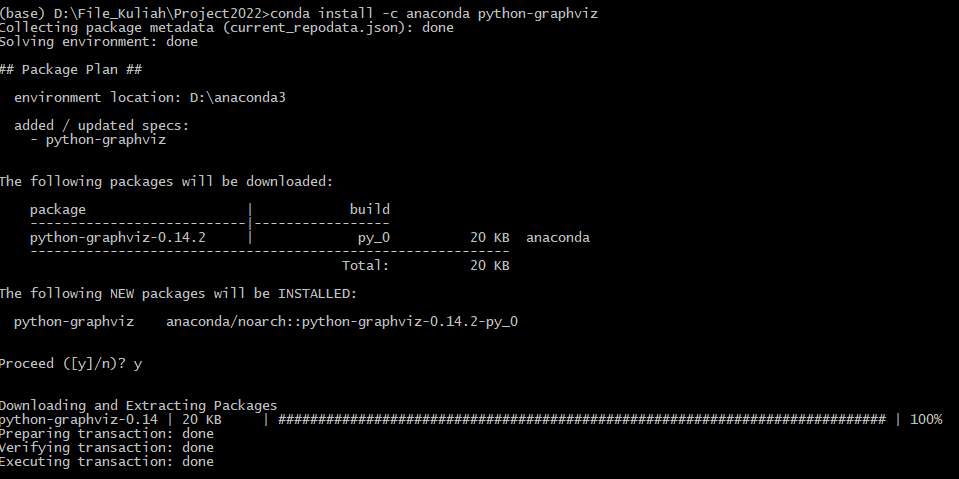
\includegraphics[width=10cm,height=6cm]{figures/solusi1-2_fix.png}
			\caption{Solusi 2}
			\label{penanda}
		\end{figure}
	\end{enumerate}